%UNDERSTANDING MULTIPLICATION - WORKSHEET 0 (IN-CLASS INSTRUCTION)
\documentclass[12pt, letterpaper, fleqn]{article}

% ----------------------------------------------------------
% PACKAGES
% ----------------------------------------------------------
\usepackage{graphicx}
\usepackage{xcolor}
\usepackage[most]{tcolorbox}
\usepackage{amsmath, amssymb}
\usepackage{fancyhdr}
\usepackage[utf8]{inputenc}
\usepackage[T1]{fontenc}
\usepackage{enumitem}
\usepackage{geometry}
\usepackage{tikz}
\usepackage{needspace}
\usepackage{multicol}

\usetikzlibrary{arrows.meta, calc, shapes.geometric}

% ----------------------------------------------------------
% PAGE SETUP
% ----------------------------------------------------------
\usepackage{times}
\geometry{letterpaper, top=1.25in, bottom=1.25in, marginpar=0.5in}

% ----------------------------------------------------------
% HEADER / FOOTER
% ----------------------------------------------------------
\newcommand{\logowidth}{3cm}
\setlength{\headheight}{20pt}
\setlength{\footskip}{40pt}

\pagestyle{fancy}
\fancyhf{}
\fancyhead[C]{\small\bfseries Understanding Multiplication}
\fancyfoot[L]{\raisebox{2pt}{
\includegraphics[width=\logowidth]{../kss.png}}}
\fancyfoot[C]{\thepage}
\fancyfoot[R]{3.1.0}

\renewcommand{\footrulewidth}{0.2pt}

% ----------------------------------------------------------
% THEME COLOR
% ----------------------------------------------------------
\definecolor{customteal}{HTML}{2fbdb9}

% ----------------------------------------------------------
% HELPER MACROS
% ----------------------------------------------------------
\newcommand{\blank}{\underline{\hspace{2.2cm}}}
\newcommand{\blanklong}{\underline{\hspace{6.5cm}}}
\newcommand{\blankshorter}{\underline{\hspace{1.5cm}}}

% ----------------------------------------------------------
% DOCUMENT
% ----------------------------------------------------------
\begin{document}

\textbf{Name:} \underline{\hspace{5cm}}
\hfill
\textbf{Date:} \underline{\hspace{3cm}}\\

\begin{tcolorbox}[colback=customteal!20]
    \large\textcolor{black}{\textbf{Introduction: What is Multiplication?}}
\end{tcolorbox}

\vspace{3mm}
\noindent
Multiplication is a fast way to do **repeated addition** when we have **equal groups**. 
Instead of adding $3 + 3 + 3 + 3 = 12$, we can write:
\[
4 \times 3 = 12
\]
This means: **4 groups of 3 objects**.

\vspace{4mm}
\begin{tcolorbox}[colback=white, colframe=black!25, boxrule=0.6pt, arc=4mm]
\textbf{Visual Representation: Equal Groups}
\begin{center}
\begin{tikzpicture}[scale=0.8]
\draw[thick, fill=customteal!10] (0,0) circle (1.2);
\draw[thick, fill=customteal!10] (3,0) circle (1.2);
\draw[thick, fill=customteal!10] (6,0) circle (1.2);
\foreach \i in {1,2,3,4} {
  \fill[red] (\i*90-45:0.6) circle (0.15);
  \fill[red] (3 + \i*90-45:0.6) circle (0.15);
  \fill[red] (6 + \i*90-45:0.6) circle (0.15);
}
\node at (0,-1.5) {Group 1 (4)};
\node at (3,-1.5) {Group 2 (4)};
\node at (6,-1.5) {Group 3 (4)};
\end{tikzpicture}
\end{center}
\noindent
Here, we have **3 groups** and **4 dots** in each group.
\[
3 \times 4 = 12
\]
\end{tcolorbox}

\newpage
\begin{tcolorbox}[colback=customteal!20]
    \large\textcolor{black}{\textbf{Guided Practice: Groups to Equations}}
\end{tcolorbox}

\vspace{4mm}
\noindent
For each drawing, write the repeated addition and the multiplication equation.

\vspace{5mm}
\begin{enumerate}[itemsep=2.5cm, leftmargin=0.6cm]
\item 
\begin{tikzpicture}[scale=0.6]
\draw[thick] (0,0) rectangle (2,2);
\draw[thick] (3,0) rectangle (5,2);
\fill[blue] (0.5, 0.5) circle(0.2); \fill[blue] (1.5, 1.5) circle(0.2);
\fill[blue] (3.5, 0.5) circle(0.2); \fill[blue] (4.5, 1.5) circle(0.2);
\end{tikzpicture}
\\
Repeated addition: \blanklong \\
Multiplication: \blank $\times$ \blank $=$ \blank

\item 
\begin{tikzpicture}[scale=0.6]
\draw[thick] (0,0) circle(1);
\draw[thick] (2.5,0) circle(1);
\draw[thick] (5,0) circle(1);
\fill[orange] (-0.3,0) circle(0.15); \fill[orange] (0.3,0) circle(0.15); \fill[orange] (0,0.4) circle(0.15);
\fill[orange] (2.2,0) circle(0.15); \fill[orange] (2.8,0) circle(0.15); \fill[orange] (2.5,0.4) circle(0.15);
\fill[orange] (4.7,0) circle(0.15); \fill[orange] (5.3,0) circle(0.15); \fill[orange] (5,0.4) circle(0.15);
\end{tikzpicture}
\\
Repeated addition: \blanklong \\
Multiplication: \blank $\times$ \blank $=$ \blank
\end{enumerate}

\newpage
\begin{tcolorbox}[colback=white!15, colframe=black, boxrule=1.5pt, arc=4mm]
\textbf{Deeper Thinking: Draw Your Own Array}
\end{tcolorbox}

\vspace{4mm}
\noindent
An **array** organizes items into equal **rows** and **columns**.
\begin{itemize}
    \item **Rows** go side-to-side (horizontal).
    \item **Columns** go up and down (vertical).
\end{itemize}

\vspace{3mm}
\noindent
Draw an array showing **3 rows and 5 columns** of stars.

\vspace{6cm}

\noindent
Write the multiplication equation for your array: \blank $\times$ \blank $=$ \blank

\end{document}
